\section{Options, final settlement, and delivery}
\label{sec:delivery}

\subsection{An option changes the cash convention}

A premium-style option purchase has a premium cash outflow, unlike entry into an ordinary future. The normal premium calculation uses the rounded monetary premium per option multiplied by signed quantity. Futures-style options have different premium and variation treatment; those conventions must not be merged \citep{CMEMoney}.

Let a premium-style call have strike $K$, one underlying future per option, and value factor $m$. Its idealized terminal intrinsic value is $m(F-K)_+$ per option. That value does not specify the operational form of settlement. For an option that exercises into a future, a long call produces a long underlying future at strike, and a long put produces a short future at strike. Their assigned counterparties receive the opposite futures positions. CME's ES option chapter defines an option on one ES future and distinguishes series with different exercise characteristics \citep{CME358A}. The appropriate series must be part of the contract state.

For accepted exercises and assignments, a compact position map is
\begin{equation}
 \Delta z^{\rm fut}=n_{LC}-n_{SC}-n_{LP}+n_{SP},
\end{equation}
where the four nonnegative counts denote long calls exercised, short calls assigned, long puts exercised, and short puts assigned. Each resulting future has its own strike transaction. Different strikes must be retained separately in the variation calculation.

\begin{example}[Exercise is an entry into the futures ledger]\label{ex:option}
Buy two premium-style calls on ES, each at a premium of 18.00 points and strike 6,000. The premium paid is $2\cdot50\cdot18=\$1,800$. Suppose both are validly exercised, each creating a long ES future at 6,000, and the relevant subsequent futures mark is 6,030. The new futures produce
\begin{equation}
 2[\nu(6030)-\nu(6000)]=\$3,000
\end{equation}
of variation. Net cash through that mark, before margin, financing, and fees, is \$1,200. There are still two futures positions unless they are closed or finally settled. Closing both at exactly 6,030 adds no further gain relative to that mark.
\end{example}

Adding both a separate \$3,000 intrinsic-value payment and the \$3,000 futures variation would double count the same economic value in this exercise convention. Conversely, recording only the option's disappearance would omit the new futures positions and their margin and expiry obligations.

Option exercise may change portfolio risk sharply. A model that approximates the option before exercise by a fractional delta must still convert an actual exercised contract into its specified integer futures position. Risk-factor nonlinearity and contract-count discreteness are different sources of nonlinearity.

\subsection{Cash-settled futures at expiry}

For a cash-settled future, final settlement closes the remaining valuation obligation through the contract's final-price rule. ES uses a special opening quotation of its underlying index, subject to the rulebook's exceptions \citep{CME358}. It is not simply the last futures trade or the previous afternoon's daily settlement.

For a position $z$ already marked to $s_{T-1}$, the final variation is
\begin{equation}
 z[\nu(s_T^{\rm final})-\nu(s_{T-1})].
\end{equation}
The settlement transition then removes the expired position. The ledger should preserve the sequence: determine the final reference, calculate the remaining variation, and discharge the contract. Removing the position before calculating the final variation would lose the last cash flow.

\subsection{Physical delivery introduces a second resource system}

The NYMEX CL contract specifies nominal units of 1,000 barrels and physical delivery at Cushing under the contract's grade, location, and procedural requirements \citep{NYMEX200}. A financial position near expiry therefore interacts with physical capacity, documentation, and payment resources. For a simplified nominal-unit planning model, $n$ long contracts require capacity to receive $1000n$ barrels and fund the invoice. A short position requires deliverable supply or another contractually valid resolution. Actual permitted tolerances and procedures remain governed by the rulebook.

A physical planning problem can be written
\begin{equation}
 Dv\le h,\qquad Ev=r(z),
\end{equation}
where $v$ allocates eligible physical resources, $h$ records capacities, and $r(z)$ records obligations generated by the expiring position. The structure resembles implied-liquidity constraints, but the resources, deadlines, and legal requirements are different. A warehouse balance, a pipeline right, and a cash balance should not be collapsed into one scalar ``liquidity'' variable.

The futures position can be financially marked before delivery completes. The delivery invoice is an additional asset-for-cash transaction, not a second payment of cumulative futures P\&L. A combined futures-and-physical ledger must include both and retain their signs.

\subsection{Treasury conversion factors and delivery choice}

For the CBOT Treasury note contract in Chapter 19, the delivery invoice uses the specified futures settlement price $F$, a conversion factor $c_k$ for deliverable $k$, and accrued interest $a_k$. Per contract,
\begin{equation}
 \mathrm{Invoice}_k(F)=\mathcal R_{0.01}(1000Fc_k)+a_k.
\label{eq:invoice}
\end{equation}
The source specifies the relevant notice-day price and the deliverable basket \citep{CBOT19}. Our example fixes a single permissible delivery date and compares synthetic eligible securities; it does not identify a currently cheapest actual Treasury.

Let $P_k$ be the clean acquisition price in points on that date, and assume acquisition and delivery use the same accrued interest. Ignoring cent rounding temporarily, acquisition cost minus invoice is
\begin{equation}
 N_k(F)=1000(P_k-Fc_k).
\label{eq:ctd}
\end{equation}
Accrued interest cancels in this fixed-date comparison. Financing, coupons received during a holding period, repo terms, transaction costs, and timing choices would change the comparison if acquisition occurs earlier.

\begin{proposition}[A delivery envelope]
On a fixed finite deliverable set with $P_k,c_k$ held constant, $N(F)=\min_kN_k(F)$ is continuous, piecewise affine, and concave. A switch between two distinct conversion factors can occur only at
\begin{equation}
 F_{ij}=\frac{P_i-P_j}{c_i-c_j}.
\end{equation}
Not every pairwise intersection lies on the lower envelope.
\end{proposition}
\begin{proof}
The minimum of finitely many affine functions is a continuous concave piecewise-affine function. A pair can exchange order only where its two affine values agree, giving the stated expression. Other deliverables may have smaller values at that point.
\end{proof}

\begin{table}[htbp]
\centering\small
\begin{tabular}{@{}lrrrrr@{}}
\toprule
Deliverable & Clean price & Factor & Accrued & Invoice at 110 & Net cost\\
\midrule
A & 99.00 & 0.9000 & \$600 & \$99,600 & \$0\\
B & 101.00 & 0.9200 & \$800 & \$102,000 & $-\$200$\\
C & 98.00 & 0.8800 & \$500 & \$97,300 & \$1,200\\
\bottomrule
\end{tabular}
\caption{A fixed-date synthetic delivery comparison. Net cost is acquisition including accrued interest minus invoice. B minimizes that cost at $F=110$; A and B cross at $F=100$.}
\label{tab:delivery}
\end{table}

The negative delivery cost for B is a comparison at the given invoice price. Total economics also include the short futures position's entry and variation history. It is not by itself a trading-profit claim. The envelope describes the seller's delivery choice conditional on these inputs; modeling the futures price requires the broader carry and option problem.

\begin{figure}[htbp]
\centering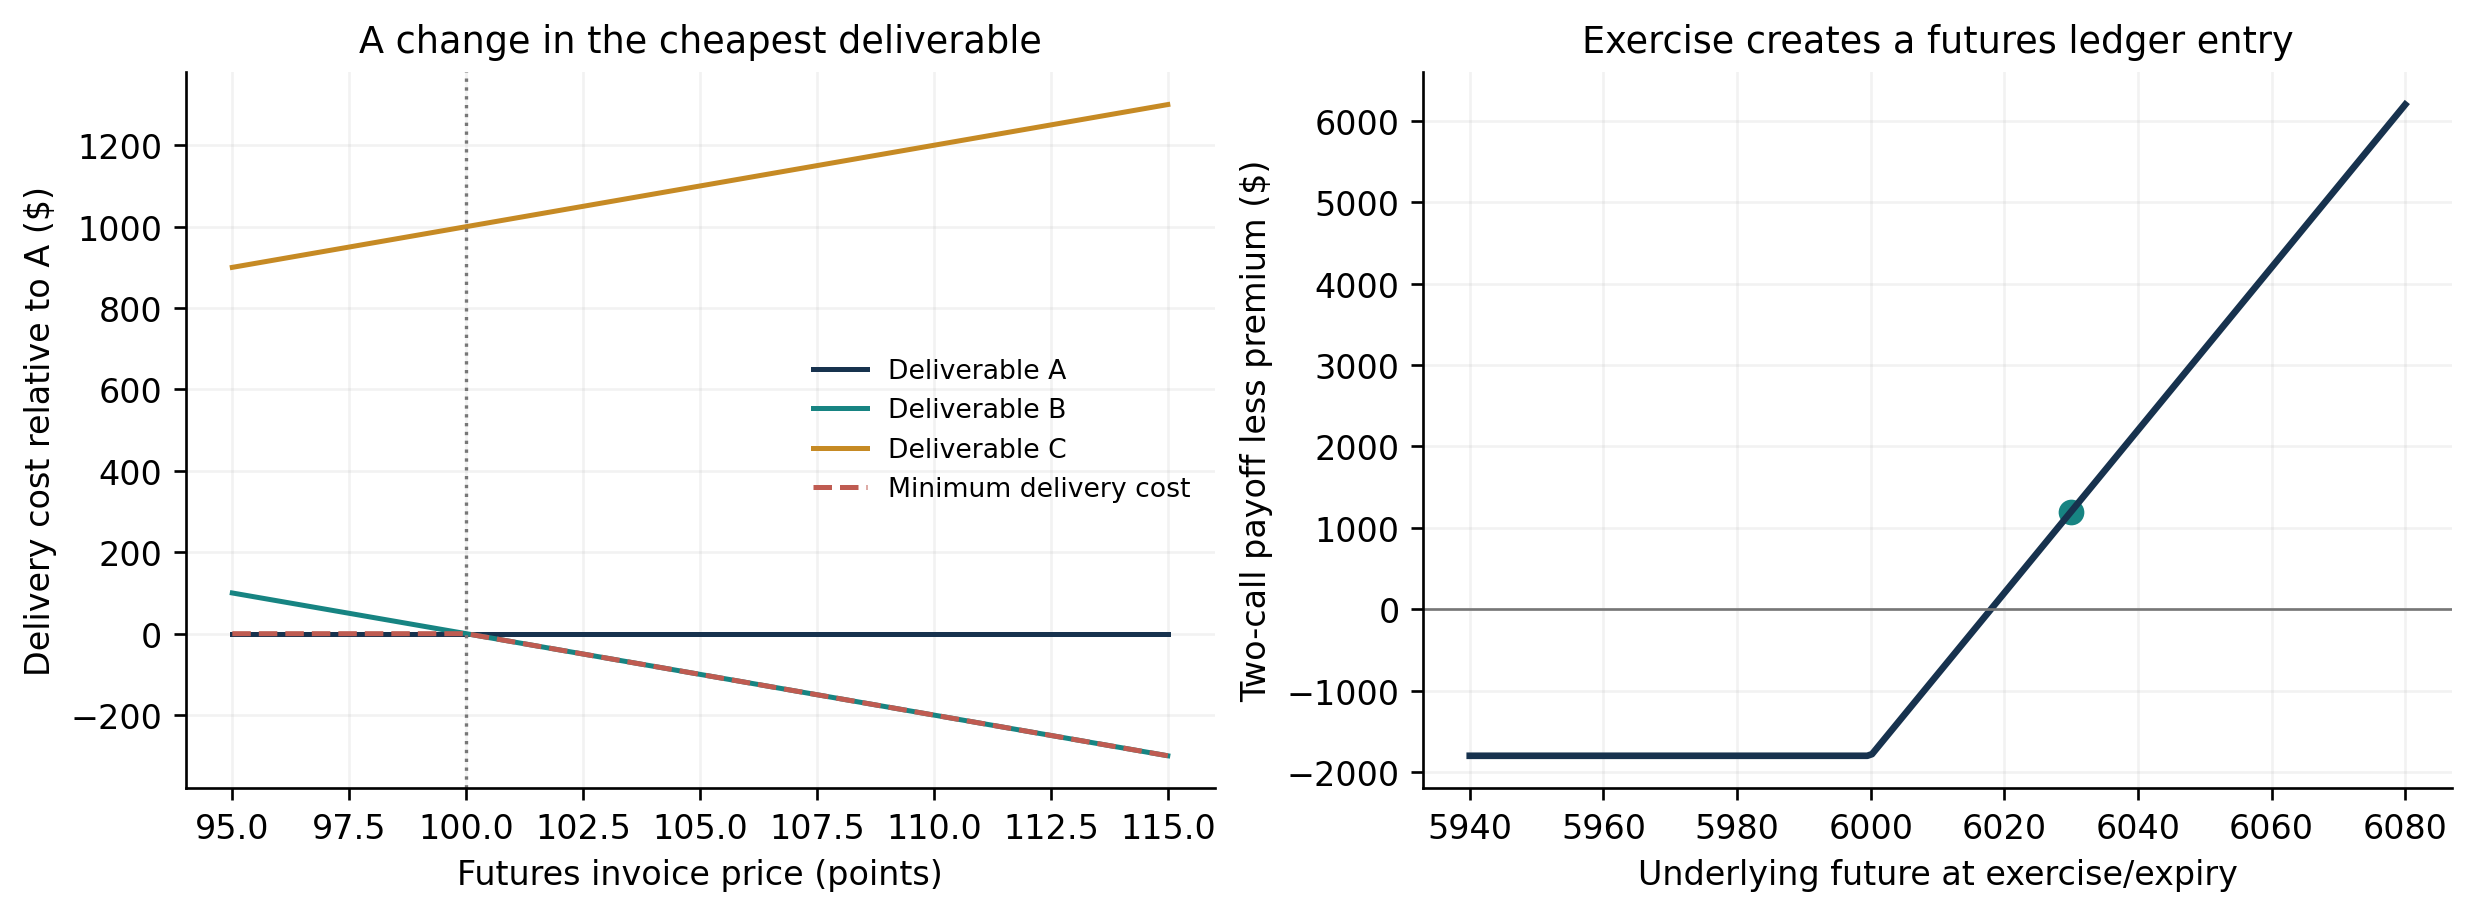
\includegraphics[width=\textwidth]{figures/09_delivery_options.png}
\caption{Two terminal maps. Left: synthetic delivery costs relative to deliverable A, preserving the identity of the cheapest security. Right: the intrinsic payoff less premium for the two calls in Example~\ref{ex:option}, assuming exercise or expiration and liquidation of any resulting futures at the displayed underlying value. Operational exercise conventions are specified separately from this payoff graph.}
\label{fig:delivery}
\end{figure}
